\section*{Appendix (Reviewers version only)}

\begin{proof}[of Claim~\ref{claim:binary_to_permutation_avoiding}]
    Let us first show that the image of $\BINTOPERM$ contains only
    permutations avoiding $213$ and $231$. Let $u$ be a binary word,
    $\pi = \BINTOPERM(u)$, and $P_0$ (resp. $P_1$) be the set of the
    positions of the occurrences of $0$ (resp. $1$) in $u$. By
    definition of $\BINTOPERM$, from left to right, the subword
    $v = \pi_{|P_0}$ is increasing and the subword $w = \pi_{|P_1}$
    is decreasing, and all letters of $w$ are greater than those
    of~$v$. Now, assume that $\pi$ admits an occurrence of $213$.
    Then, since $v$ is increasing and $w$ is decreasing, there is an
    occurrence of $3$ (resp. $13$, $23$) in $v$ and a relative
    occurrence of $21$ (resp. $2$, $1$). All these three cases
    contradict the fact that all letters of $w$ are greater than
    those of $v$. A similar argument shows that $\pi$ avoids~$231$
    as well.
    \smallskip

    Finally, observe that any permutation $\pi$ avoiding $213$ and
    $231$ necessarily starts by the smallest possible letter or the
    greatest possible letter. This property is then true for the
    suffix of $\pi$ obtained by deleting its first letter,
    and so on for all of its suffixes. Thus, by
    replacing each letter $a$ of $\pi$ by $0$ (resp. $1$) if $a$ has the
    role of a smallest (resp. greatest) letter, one obtains a binary
    word $u$ such that $\BINTOPERM(u) = \pi$. Hence, all permutations
    avoiding $213$ and $231$ are in the image of $\BINTOPERM$.
    \qed
\end{proof}
\bigskip

\begin{proof}[of Claim~\ref{claim:square_binary_to_square_permutation}]
    Since $u$ is a square binary word, there is a binary word $v$
    such that $u \in v \shuffle v$. Then, there are two disjoint
    sets $P$ and $Q$ of positions of letters of $u$ such that
    $u_{|P} = v = u_{|Q}$. Now, by definition of $\BINTOPERM$, the
    words $\BINTOPERM(u)_{|P}$ and $\BINTOPERM(u)_{|Q}$ have the
    same standardized $\sigma$. Hence, and by definition of
    the shuffle product of permutations, $\BINTOPERM(u)$ appears in
    $\sigma \SHUFFLE \sigma$, showing that $\BINTOPERM(u)$ is a
    square permutation.
    \qed
\end{proof}
\bigskip

\begin{proof}[of Claim~\ref{claim:square_permutation_to_square_binary}]
    Let $\pi$ be a square permutation avoiding $213$ and $231$. By
    Claim~\ref{claim:binary_to_permutation_avoiding}, $\pi$ is in
    the image of $\BINTOPERM$ and hence, $u = \PERMTOBIN(\pi)$ is a
    well-defined binary word. Since $\pi$ is a square permutation,
    there are two disjoint sets $P_1$ and $P_2$ of indexes of letters
    of $\pi$ such that $\pi_{|P_1}$ and $\pi_{|P_2}$ are
    order-isomorphic. This implies, by the definitions of $\BINTOPERM$
    and $\PERMTOBIN$, that $u_{|P_1} = u_{|P_2}$, showing that $u$
    is a square binary word.
    \qed
\end{proof}
\bigskip

\begin{proof}[of Lemma~\ref{lem:endomorphisms}]
    To prove, for $j = 1, 2, 3$, that $\phi_j$ is a morphism of
    associative algebras, we have to prove that for all permutations
    $\sigma$ and $\nu$,
    \begin{equation}
        \phi_j(\sigma \SHUFFLE \nu) =
        \phi_j(\sigma) \SHUFFLE \phi_j(\nu).
    \end{equation}
    We shall proceed here as we have done during the proof of
    Proposition~\ref{prop:shuffle_associative_commutative} by showing
    that $\phi_j$ is a morphism of coalgebras, that is
    \begin{equation}
        \Delta \phi_j = (\phi_j \otimes \phi_j) \Delta.
    \end{equation}
    In the sequel, $\pi$ is a permutation.
    \smallskip

    If $P$ is a set of indexes of letters of $\pi$, we denote by
    $\widetilde{P}$ the set $\{|\pi| - i  + 1 : i \in P\}$. Now, since
    the operation $\widetilde{\,}$ defines a bijection on the set of the
    subsets of $[|\pi|]$, and since the standardization operation
    commutes with the mirror operation on words without multiple
    occurrence of a letter, we have
    \begin{equation} \begin{split}
        \Delta(\phi_1(\pi))
        & = \sum_{P_1 \sqcup P_2 = [|\pi|]}
        \STD\left(\phi_1(\pi)_{|P_1}\right)
        \otimes \STD\left(\phi_1(\pi)_{|P_2}\right) \\
        & = \sum_{P_1 \sqcup P_2 = [|\pi|]}
        \STD\left(\widetilde{\pi}_{|P_1}\right)
        \otimes \STD\left(\widetilde{\pi}_{|P_2}\right) \\
        & = \sum_{P_1 \sqcup P_2 = [|\pi|]}
        \STD\left(\widetilde{\pi}_{|\widetilde{P_1}}\right)
        \otimes \STD\left(\widetilde{\pi}_{|\widetilde{P_2}}\right) \\
        & = \sum_{P_1 \sqcup P_2 = [|\pi|]}
        \widetilde{\STD\left(\pi_{|P_1}\right)}
        \otimes \widetilde{\STD\left(\pi_{|P_2}\right)} \\
        & = \sum_{P_1 \sqcup P_2 = [|\pi|]}
        \phi_1\left(\STD\left(\pi_{|P_1}\right)\right)
        \otimes \phi_1\left(\STD\left(\pi_{|P_2}\right)\right) \\
        & = (\phi_1 \otimes \phi_1) \Delta(\pi).
    \end{split} \end{equation}
    This shows that $\phi_1$ is a morphism of coalgebras and hence, that
    $\phi_1$ is a morphism of associative algebras.
    \smallskip

    Next, since by definition of the complementation operation on
    permutations, for any permutation $\tau$ and any indexes $i$ and $k$,
    we have $\tau(i) < \tau(k)$ if and only if $\bar \tau(i) > \bar \tau(k)$,
    we have
    \begin{equation} \begin{split}
        \Delta(\phi_2(\pi))
        & = \sum_{P_1 \sqcup P_2 = [|\pi|]}
        \STD\left(\phi_2(\pi)_{|P_1}\right)
        \otimes \STD\left(\phi_2(\pi)_{|P_2}\right) \\
        & = \sum_{P_1 \sqcup P_2 = [|\pi|]}
        \STD\left(\bar \pi_{|P_1}\right)
        \otimes \STD\left(\bar \pi_{|P_2}\right) \\
        & = \sum_{P_1 \sqcup P_2 = [|\pi|]}
        \phi_2\left(\STD\left(\pi_{|P_1}\right)\right)
        \otimes \phi_2\left(\STD\left(\pi_{|P_2}\right)\right) \\
        & = (\phi_2 \otimes \phi_2) \Delta(\pi).
    \end{split} \end{equation}
    This shows that $\phi_2$ is a morphism of coalgebras and hence, that
    $\phi_2$ is a morphism of associative algebras.
    \smallskip

    Finally, for any permutation $\tau$, if $P$ is a set of indexes of
    letters of $\tau$, we denote by $P_\tau^{-1}$ the set
    $\{\tau(i) : i \in P\}$. Since the map sending a subset $P$ of
    $[|\pi|]$ to $P_\pi^{-1}$ is a bijection, and since
    $\STD\left(\pi_{|P}\right)^{-1} = \STD\left(\pi^{-1}_{|P_\pi^{-1}}\right)$,
    we have
    \begin{equation} \begin{split}
        \Delta(\phi_3(\pi))
        & = \sum_{P_1 \sqcup P_2 = [|\pi|]}
        \STD\left(\phi_3(\pi)_{|P_1}\right)
        \otimes \STD\left(\phi_3(\pi)_{|P_2}\right) \\
        & = \sum_{P_1 \sqcup P_2 = [|\pi|]}
        \STD\left(\pi^{-1}_{|P_1}\right)
        \otimes \STD\left(\pi^{-1}_{|P_2}\right) \\
        & = \sum_{P_1 \sqcup P_2 = [|\pi|]}
        \STD\left(\pi^{-1}_{|{P_1}_\pi^{-1}}\right)
        \otimes \STD\left(\pi^{-1}_{|{P_2}_\pi^{-1}}\right) \\
        & = \sum_{P_1 \sqcup P_2 = [|\pi|]}
        \STD\left(\pi_{|P_1}\right)^{-1}
        \otimes \STD\left(\pi_{|P_2}\right)^{-1} \\
        & = \sum_{P_1 \sqcup P_2 = [|\pi|]}
        \phi_3\left(\STD\left(\pi_{|P_1}\right)\right)
        \otimes \phi_3\left(\STD\left(\pi_{|P_2}\right)\right) \\
        & = (\phi_3 \otimes \phi_3) \Delta(\pi).
    \end{split} \end{equation}
    This shows that $\phi_3$ is a morphism of coalgebras and hence, that
    $\phi_3$ is a morphism of associative algebras.
    \qed
\end{proof}
\bigskip

\begin{proof}[of Lemma~\ref{lemma:matching}]
    The proof is, naturally enough, a slight extension of
    Lemma~1 in \cite{Rizzi:Vialette:CSR:2013} and is added here in full
    for the sake of completeness.

    (\emph{1} $\Rightarrow$ \emph{2}).
    Since $\pi$ is a square, it admits a square root $\sigma$.
    Let $2n = |\pi|$ (and hence
    $|\sigma| = n$).
    By definition, there are two sets $I^1 = \{i^1_1 < i^1_2 < \dots < i^1_n\}$
    and $I^2 = \{i^2_1 < i^2_2 < \dots < i^2_n\}$ of disjoint indexes of
    $\pi$ such that $\pi_{|I^1}$ and $\pi_{|I^2}$ are both
    order-isomorphic to $\sigma$.
    Let $K_\pi$ be the linear clique associated with $\pi$ with vertices
    $\VS{K_\pi} = \{i^1_j : j \in [n]\} \cup \{i^2_j : j \in [n]\}$. It
    is easily seen that $\mathcal{M} = \{\{i^1_j, i^2_j\} : j \in [n]\}$
    is a subset of $\ES{K_\pi}$. Furthermore, $\mathcal{M}$ is a perfect
    matching since $I^1 \cap I^2 = \emptyset$, and
    $I^1 \cup I^2 = \{1, 2,  \dots 2n\}$. It is also containment-free.
    Indeed, if it is not the case then there would exist two edges
    $e = \{i^1_j, i^2_j\}$ and $e' = \{i^1_k, i^2_k\}$, $j < k$, in
    $\mathcal{M}$ such that $i^1_j < i^1_k < i^2_k < i^2_j$ or
    $i^1_j < i^2_k < i^1_k < i^2_j$. This is a contradiction since
    $i^2_k > i^2_j$ if $k > j$. Finally, for any two distinct edges
    $e = \{\i^1_j, i^2_j\}$ and $e' = \{i^1_k, i^2_k\}$ of $\mathcal{M}$,
    we have $\pi(i^1_j) < \pi(i^2_j)$ if and only if
    $\pi(i^1_k) < \pi(i^2_k)$ since we are comparing in both cases two
    elements (at position $j$ and $k$) in two patterns that are
    order-isomorphic to $\sigma$.

    (\emph{2} $\Rightarrow$ \emph{1}).
    Let $I^1 = \{i^1_j : \exists \{i_j, i_k\} \in \mathcal{M}
    \;\text{with}\; j < k\}$, and
    $I^2 = \{i^2_k : \exists \{i_j, i_k\} \in \mathcal{M}
    \;\text{with}\; j < k\}$.
    Informally, $I^1$ (resp. $I^2$) is the set of the left (resp. right)
    endpoints of the edges in $\mathcal{M}$ assuming the positions
    $1, 2, \dots, 2$ are drawn along an horizontal line.
    Without loss of generality, assume $i^1_1 < i^1_2 < \dots < i^1_n$.
    % and $I^2 = \{i^2_1, i^2_2, \dots, i^2_n\}$.
    Let $p^1 = \pi(i^1_1) \pi(i^1_2) \dots \pi(i^1_n)$ and
    $p^2 = \pi(i^2_1) \pi(i^2_2) \dots \pi(i^2_n)$ be the two patterns
    from $\pi$ induced by $I^1$ and $I^2$, respectively. Clearly $p^1$
    and $p^2$ are disjoint in $\pi$ (since $\mathcal{M}$ is a matching)
    and cover $\pi$ (since $\mathcal{M}$ is perfect). We also claim that
    $p^1$ and $p^2$ are order-isomorphic. Suppose, aiming at a
    contradiction, that this is not the case. Therefore, there exist two
    positions $j$ and $k$, say $j < k$, such that
    $\pi(i^1_j) < \pi(i^2_j)$ and $\pi(i^1_k) > \pi(i^2_k)$, or
    $\pi(i^1_j) < \pi(i^2_j)$ and $\pi(i^1_k) > \pi(i^2_k)$.
    But since $\mathcal{M}$ is containment-free, it follows that both
    $\{i^1_j, i^2_j\}$, $i^1_j < i^2_j$, and $\{i^1_k, i^2_k\}$,
    $i^1_k, i^2_k$, belong to $\mathcal{M}$. This is a contradiction
    since for any two distinct edges $(a, b)$ and $(a', b')$ in
    $\mathcal{M}$ we have $\pi(a) < \pi(a')$ if and only if
    $\pi(b) < \pi(b')$.
    \qed
\end{proof}
\bigskip

\begin{proof}[of Lemma~\ref{lemma:at most one edge monotone}]
  We first prove \emph{1}. Suppose, aiming at a contradiction, that
  there exist two $(\sigma_1, \sigma_2)$-edges $(a, a')$ and $(b, b')$
  in $\mathcal{M}$. Since $\mathcal{M}$ is containment-free, we may
  assume $a < b$ and $a' < b'$. Therefore, we have $\pi(a) < \pi(b)$
  (since $\sigma_1$ is increasing) and $\pi(a') > \pi(b')$ (since
  $\sigma_2$ is decreasing), which contradicts our hypothesis about
  $\mathcal{M}$.

  As for \emph{2}, suppose, still aiming at a contradiction, that there
  exist two $(\sigma_1, \sigma_2)$-edges $(a, a')$ and $(b, b')$ in
  $\mathcal{M}$. Since $\mathcal{M}$ is containment-free, we may assume
  $a < b$ and $a' < b'$. Therefore, we have $\pi(a) > \pi(b)$ (since
  $\sigma_1$ is decreasing) and $\pi(a') < \pi(b')$ (since $\sigma_2$ is
  increasing), which contradicts our hypothesis about~$\mathcal{M}$.
  \qed
\end{proof}

\bigskip

\begin{proof}[of Proposition~\ref{proposition:hardness}]
  Suppose first that $\sigma$ occurs in $\pi$ and fix an occurrence.
  Construct a matching $\mathcal{M}$ as follows:
  \begin{itemize}
    \item $\mathcal{M}$ contains $N_1$ pairwise crossing
    $(\nu_1, \nu'_1)$-edges.
    \item $\mathcal{M}$ contains $N_2$ pairwise crossing
    $(\nu_2, \nu'_2)$-edges.
    \item $\mathcal{M}$ contains $N_3$ pairwise crossing
    $(\nu_3, \nu'_3)$-edges.
    \item $\mathcal{M}$ contains $N_4$ pairwise crossing
    $(\nu_4, \nu'_4)$-edges.
    \item $\mathcal{M}$ contains $k+2$ pairwise crossing
    $(\sigma', \pi')$-edges as depicted in
    Figure~\ref{fig:subfig:sigma' - pi' - pi'' - sigma''}.
    More precisely,
    (i) the first position of $\sigma'$
    (\emph{i.e.}, $(2N_1+N_2+N_3) + 1$) is linked
    to the first position of $\pi'$
    (\emph{i.e.}, $(2N_1 + 2N_2 + 2N_3 + N_4 + k + 2) + 1$),
    (ii) the last position of $\sigma'$
    (\emph{i.e.}, $(2N_1+N_2+N_3) + k+2$) is linked
    to the last position of $\pi'$
    (\emph{i.e.}, $(2N_1 + 2N_2 + 2N_3 + N_4 + k + 2) + n+2$),
    and all other positions in $\sigma'$ are linked by means of $k$ pairwise
    crossing edges to the positions in
    $\pi'$ that correspond to the fixed occurence of $\sigma$ in $\pi$.
    (Notice that we use here the fact that $\sigma$ occurs in $\pi$).
    \item $\mathcal{M}$ contains $n-k$ pairwise crossing
    $(\pi', \pi'')$-edges as depicted in
    Figure~\ref{fig:subfig:sigma' - pi' - pi'' - sigma''}.
    More precisely,
    all positions in $\pi'$ that do not correspond to the fixed occurence of
    $\sigma$ in $\pi$ are linked by means of $n-k$ pairwise crossing edges
    to the positions in $\pi''$ that do not correspond to the fixed
    occurrence of $\sigma$ in $\pi$.
    \item $\mathcal{M}$ contains $k$ pairwise crossing
    $(\pi'', \sigma'')$-edges as depicted in
    Figure~\ref{fig:subfig:sigma' - pi' - pi'' - sigma''}.
    More precisely, the positions in $\pi''$ that correspond to
    the fixed occurrence of $\sigma$ in $\pi$ are linked
    by means of $k$ pairwise crossing edges to all positions in
    $\sigma''$.
    (Notice that we use here the fact that $\sigma$ occurs in $\pi$).
  \end{itemize}
  It can be easily checked (probably referring to Figure~\ref{fig:reduction}) that
  $\mathcal{M}$ is perfect, containment-free and that
  for any two disctinct edges
  $(a, b)$ and $(a', b')$ in $\mathcal{M}$
  we have $\mu(a) < \mu(a')$ if and only if $\mu(b) < \mu(b')$.


    \begin{figure}[t!]
      \centering
        \begin{tikzpicture}
          [
            scale=0.35,
            label/.style={anchor=base},
            cell/.style={draw,thick,fill=black!5}
          ]
          % sigma'
          \draw [cell,rounded corners] (1.5,16.5) -- (4.5,16.5) -- (4.5,19.5) -- (1.5,19.5) -- cycle;
          \draw[step=1cm,black!60,ultra thin,fill=black!10] (0.8,16.8) grid (5.2,21.2);
          \foreach \x/\y in {1/20,2/19,3/17,4/18,5/21} {
              \draw [fill=black] (\x,\y) circle (0.1);
          }
          \node (pip) at (3,22) {$\sigma'$};
          \node[%
            draw,
            text width=5.5cm,text justified,color=black!50,rounded corners,
            rectangle callout,callout relative pointer={(0.0cm,-1cm)}
          ] at (3,26)
          {%
            $((k+1) \; \sigma \; (k+2)) \; [2N_2 + N_4 + 2n + k + 2]$
          };%
          %\node at (3,-0.5) {$((k+1) \; \sigma \; (k+2)) \; [2N_2 + N_4 + 2n + k + 2]$};
          \node at (-0.5,20) {$k+1$};
          \node at (-0.5,21) {$k+2$};
          % pi'
          \draw [cell,rounded corners] (6.5,8.5) -- (12.5,8.5) -- (12.5,14.5) -- (6.5,14.5) -- cycle;
          \draw[step=1cm,black!60,ultra thin,fill=black!10] (5.8,8.8) grid (13.2,16.2);
          \foreach \x/\y in {6/15,7/12,8/13,9/10,10/9,11/11,12/14,13/16} {
              \draw [fill=black] (\x,\y) circle (0.1);
          }
          \node (pip) at (9.5,17) {$\pi'$};
          \node[%
            draw,
            text width=5.5cm,text justified,color=black!50,rounded corners,
            rectangle callout,callout relative pointer={(0.0cm,3.5cm)}
          ] at (9.5,-3.5)
          {%
            $((n+1) \; \pi \; (n+2)) \; [2N_2 + N_4 + n + k + 2]$
          };%
          %\node at (9.5,-2) {$((n+1) \; \pi \; (n+2)) \; [2N_2 + N_4 + n + k + 2]$};
          \node at (-0.5,15) {$n+1$};
          \node at (-0.5,16) {$n+2$};
          % pi''
          \draw [cell,rounded corners] (13.5,2.5) -- (19.5,2.5) -- (19.5,8.5) -- (13.5,8.5) -- cycle;
          \draw[step=1cm,black!60,ultra thin,fill=black!10] (13.8,2.8) grid (19.2,8.2);
          \foreach \x/\y in {14/6,15/7,16/4,17/3,18/5,19/8} {
              \draw [fill=black] (\x,\y) circle (0.1);
          }
          \node (pipp) at (16.75,9) {$\pi''$};
          \node[%
            draw,
            text width=2.25cm,text justified,color=black!50,rounded corners,
            rectangle callout,callout relative pointer={(0.0cm,-3cm)}
          ] at (16.5,19)
          {%
            $\pi [2N_2 + N_4 + k]$
          };%
          %\node at (16.5,-3.5) {$\pi [2N_2 + N_4 + k]$};
          % sigma''
          \draw [cell,rounded corners] (19.5,-0.5) -- (22.5,-.5) -- (22.5,2.5) -- (19.5,2.5) -- cycle;
          \draw[step=1cm,black!60,ultra thin,fill=black!10] (19.8,-0.2) grid (22.2,2.2);
          \foreach \x/\y in {20/2,21/0,22/1} {
              \draw [fill=black] (\x,\y) circle (0.1);
          }
          \node (sigmapp) at (21,3) {$\sigma''$};
          \node[%
            draw,
            text width=1.75cm,text justified,color=black!50,rounded corners,
            rectangle callout,callout relative pointer={(0.0cm,0.75cm)}
          ] at (21,-4.5)
          {%
            $\sigma [2N_2 + N_4]$
          };%
          %\node at (21,-5) {$\sigma [2N_2 + N_4]$};
          % edges sigma' - pi'
          \draw [line width=1pt]
          (1,20) .. controls +(0,9) and +(0,4) .. (6,15);
          \draw [line width=1pt]
          (5,21) .. controls +(0,9) and +(0,4) .. (13,16);
          \draw [line width=1pt]
          (2,19) .. controls +(0,-17) and +(0,-7) .. (8,13);
          \draw [line width=1pt]
          (3,17) .. controls +(0,-17) and +(0,-7) .. (9,10);
          \draw [line width=1pt]
          (4,18) .. controls +(0,-17) and +(0,-7) .. (11,11);
          % edges pi' - pi''
          \draw [line width=1pt]
          (7,12) .. controls +(0,9) and +(0,4) .. (14,6);
          \draw [line width=1pt]
          (10,9) .. controls +(0,9) and +(0,4) .. (17,3);
          \draw [line width=1pt]
          (12,14) .. controls +(0,9) and +(0,4) .. (19,8);
          % edges pi'' - sigma''
          \draw [line width=1pt]
          (15,7) .. controls +(0,-9) and +(0,-4) .. (20,2);
          \draw [line width=1pt]
          (16,4) .. controls +(0,-9) and +(0,-4) .. (21,0);
          \draw [line width=1pt]
          (18,5) .. controls +(0,-9) and +(0,-4) .. (22,1);
          % text
          % \node[%
          %   draw,
          %   text width=5.5cm,text justified,color=black!50,
          %   rectangle callout,callout relative pointer={(0.5cm,-.75cm)}
          % ] at (1,27)
          % {%
          % $2$ pairwise crossing $(\sigma',\pi')$-edges that
          % link the guards
          % };%
          % \node[%
          %   draw,
          %   text width=5.5cm,text justified,color=black!50,
          %   rectangle callout,callout relative pointer={(-0.1cm,-2.5cm)}
          % ] at (17,24)
          % {%
          % $n-k$ pairwise crossing $(\sigma',\pi')$-edges that
          % denote positions that do not correspond to
          % a specific occurence of $\sigma$ in $\pi$
          % (at positions $2$, $3$ and $5$).
          % };%
          % \node[%
          %   draw,
          %   text width=5.5cm,text justified,color=black!50,
          %   rectangle callout,callout relative pointer={(0.75cm,1.5cm)}
          % ] at (2.5,4,5)
          % {%
          % $k$ pairwise crossing $(\sigma',\pi')$-edges that
          % denote a specific occurence of $\sigma$ in $\pi$
          % (at positions $2$, $3$ and $5$).
          % };%
          % \node[%
          %   draw,
          %   text width=5.5cm,text justified,color=black!50,
          %   rectangle callout,callout relative pointer={(2cm,.75cm)}
          % ] at (7,-3)
          % {%
          % $k$ pairwise crossing $(\pi''; \sigma'')$-edges that
          % denote a specific occurence of $\sigma$ in $\pi$
          % (at positions $2$, $3$ and $5$).
          % };%
        \end{tikzpicture}
        \caption{\label{fig:subfig:sigma' - pi' - pi'' - sigma''}%
        Illustration of the containment-free perfect matching $\mathcal{M}$
        between gadgets $\sigma'$, $\pi'$, $\pi''$ and $\sigma''$ assuming two
        input permutation $\sigma = 312$ and $\pi = 4\mathbf{5}\mathbf{2}1\mathbf{3}6$
        (where a specific occurrence of $\sigma$ in $\pi$ is depicted in bold).
        }
      \end{figure}

  Conversely, suppose that there exists a containment-free perfect matching
  $\mathcal{M}$ in $K_\mu$ such that for any two disctinct edges
  $(a, b)$ and $(a', b')$ in $\mathcal{M}$
  we have $\mu(a) < \mu(a')$ if and only if $\mu(b) < \mu(b')$.
  We show that $\sigma$ occurs as a pattern in $\pi$.
  Whereas the matching $\mathcal{M}$ may not be as regular as in the forward
  direction, the main idea is to prove that $\mathcal{M}$ contains enough structure
  (more precisely, $k+2$ $(\sigma', \pi')$-edges) so that we can conclude
  that $\sigma$ occurs in $\pi$.
  We have divided the reverse direction into a serie of basic claims that
  progressively defines the overall structure of $\mathcal{M}$
  (refer to Fig.~\ref{fig:reduction}).

    \begin{figure}[t!]
      \centering
      \subfigure[%
        A $(\nu_1, \nu_2)$-edge $(a, b)$ together with a
        $(\nu_2, \nu'_1)$-edge $(x, y)$.
        Notice that we may have $x<b$
        (as long as $N_1 < x \leq N_1+N_2$ and $N_1 < b \leq N_1+N_2$
        do hold).
      ]{%
        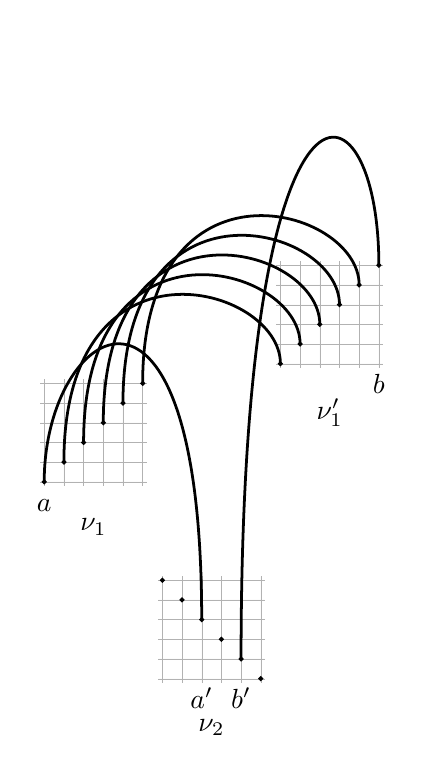
\begin{tikzpicture}
          [
            scale=0.25,
            label/.style={anchor=base}
          ]
          % nu_1
          \draw[step=1cm,black!30,ultra thin,fill=black!10] (-0.2,9.8) grid (5.2,15.2);
          \foreach \x/\y in {0/10,1/11,2/12,3/13,4/14,5/15} {
              \draw [fill=black] (\x,\y) circle (0.1);
          }
          % nu_4
          \draw[step=1cm,black!30,ultra thin,fill=black!10] (5.8,-0.2) grid (11.2,5.2);
          \foreach \x/\y in {6/5,7/4,8/3,9/2,10/1,11/0} {
              \draw [fill=black] (\x,\y) circle (0.1);
          }
          % nu'_1
          \draw[step=1cm,black!30,ultra thin,fill=black!10] (11.8,15.8) grid (17.2,21.2);
          \foreach \x/\y in {12/16,13/17,14/18,15/19,16/20,17/21} {
              \draw [fill=black] (\x,\y) circle (0.1);
          }
          % labels
          \node [label] (y) at (17,14.5) {$b$};
          \node [label] (yp) at (10,-1.5) {$b'$};
          \node [label] (a) at (0,8.5) {$a$};
          \node [label] (ap) at (8,-1.5) {$a'$};
          \node (nu1) at (2.5,7.7) {$\nu_1$};
          \node (nu2) at (8.5,-2.5) {$\nu_2$};
          \node (nu1') at (14.5,13.5) {$\nu'_1$};
          % crossings edges
          \draw [line width=1pt]
          (1,11) .. controls +(0,12) and +(0,4) .. (12,16);
          \draw [line width=1pt]
          (2,12) .. controls +(0,12) and +(0,4) .. (13,17);
          \draw [line width=1pt]
          (3,13) .. controls +(0,12) and +(0,4) .. (14,18);
          \draw [line width=1pt]
          (4,14) .. controls +(0,12) and +(0,4) .. (15,19);
          \draw [line width=1pt]
          (5,15) .. controls +(0,12) and +(0,4) .. (16,20);
          % data edges
          \draw [line width=1pt]
          (0,10) .. controls +(0,8) and +(0,20) .. (8,3);
          \draw [line width=1pt]
          (10,1) .. controls +(0,32) and +(0,10) .. (17,21);
        \end{tikzpicture}
        \label{subfig:no (nu_1, nu_2)-edge - 1}
      }% end subfigure
      \qquad
      \subfigure[%
        A $(\nu_1, \nu'_1)$-edge $(x', y')$ together with an
        edge $(y, z)$ which is neither
        a $(\nu_1, \nu'_1)$-edge,
        nor a $(\nu_2, \nu'_1)$-edge,
        nor a $(\nu'_1, \nu'_1)$-edge.
        Notice that $y$ may be any position satisfying
        $N_1+N_2 < y \leq 2N_1+N_2$.
      ]{%
      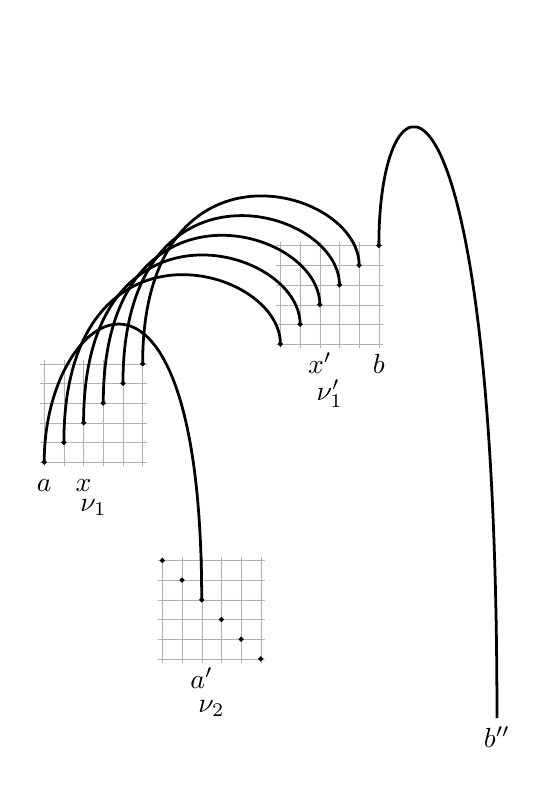
\begin{tikzpicture}
        [
          scale=0.25,
          label/.style={anchor=base}
        ]
        % nu_1
        \draw[step=1cm,black!30,ultra thin,fill=black!10] (-0.2,9.8) grid (5.2,15.2);
        \foreach \x/\y in {0/10,1/11,2/12,3/13,4/14,5/15} {
            \draw [fill=black] (\x,\y) circle (0.1);
        }
        % nu_4
        \draw[step=1cm,black!30,ultra thin,fill=black!10] (5.8,-0.2) grid (11.2,5.2);
        \foreach \x/\y in {6/5,7/4,8/3,9/2,10/1,11/0} {
            \draw [fill=black] (\x,\y) circle (0.1);
        }
        % nu'_1
        \draw[step=1cm,black!30,ultra thin,fill=black!10] (11.8,15.8) grid (17.2,21.2);
        \foreach \x/\y in {12/16,13/17,14/18,15/19,16/20,17/21} {
            \draw [fill=black] (\x,\y) circle (0.1);
        }
        % labels
        \node [label] (y) at (17,14.5) {$b$};
        \node [label] (ypp) at (23,-4.5) {$b''$};
        \node [label] (a) at (0,8.5) {$a$};
        \node [label] (a) at (2,8.5) {$x$};
        \node [label] (a) at (14,14.5) {$x'$};
        \node [label] (ap) at (8,-1.5) {$a'$};
        \node (nu1) at (2.5,7.7) {$\nu_1$};
        \node (nu2) at (8.5,-2.5) {$\nu_2$};
        \node (nu1') at (14.5,13.5) {$\nu'_1$};
        % crossings edges
        \draw [line width=1pt]
        (1,11) .. controls +(0,12) and +(0,4) .. (12,16);
        \draw [line width=1pt]
        (2,12) .. controls +(0,12) and +(0,4) .. (13,17);
        \draw [line width=1pt]
        (3,13) .. controls +(0,12) and +(0,4) .. (14,18);
        \draw [line width=1pt]
        (4,14) .. controls +(0,12) and +(0,4) .. (15,19);
        \draw [line width=1pt]
        (5,15) .. controls +(0,12) and +(0,4) .. (16,20);
        % data edges
        \draw [line width=1pt]
        (0,10) .. controls +(0,8) and +(0,20) .. (8,3);
        \draw [line width=1pt]
        (17,21) .. controls +(0,10) and +(0,35) .. (23,-3);
        \end{tikzpicture}
        \label{subfig:no (nu_1, nu_2)-edge - 2}
      }% end subfigure
      \caption{\label{fig:subfig:no (nu_1, nu_2)-edge}%
        Claim~\ref{claim:no (nu_1, nu_2)-edge}:
        Assuming a $(\nu_1,\nu_2)$-edge $(a, b)$ in $\mathcal{M}$.
      }
    \end{figure}

  \begin{claim}
    \label{claim:no (nu_1, nu_2)-edge}
    There is no $(\nu_1, \nu_2)$-edge in $\mathcal{M}$.
  \end{claim}

  \begin{proof}[of Claim~\ref{claim:no (nu_1, nu_2)-edge}]
    First, according to Lemma~\ref{lemma:at most one edge monotone},
    there exists at most one $(\nu_1, \nu_2)$-edge in $\mathcal{M}$.
    Suppose now, aiming at a contradiction, that there exists
    exactly one $(\nu_1, \nu_2)$-edge $e = (a, a')$ in $\mathcal{M}$.
    Under this assumption, we show that $\mathcal{M}$ does not contain any $(\nu_1, \nu_1)$-edge.
    Indeed, suppose, aiming at a contradiction,
    that there exists a $(\nu_1, \nu_1)$-edge $(b, b')$ in $\mathcal{M}$.
    Since $\mathcal{M}$ is containment-free,
    we must have $b < a$.
    Then it follows that $\mu(b) < \mu(a)$ (since $\nu_1$ is increasing) and
    $\mu(b') > \mu(a')$ (since $\nu_1$ is above $\nu_2$),
    which contradicts our hypothesis about $\mathcal{M}$.
    Hence $\mathcal{M}$ does not contain any $(\nu_1, \nu_1)$-edge.
    Furthermore, since $\nu_1$ is increasing and
    there exists only one $(\nu_1, \nu_2)$-edge $(a, a')$ in $\mathcal{M}$,
    we conclude that
    $\mathcal{M}$ contains $N_1-1$ pairwise crossing $(\nu_1, \nu'_1)$-edges.
    But $|\nu_1| = |\nu'_1| = N_1$ and $\mathcal{M}$ is perfect,
    and hence there exists a position, say $b$, in $\nu'_1$ that is
    not involved in a $(\nu_1, \nu'_1)$-edge in $\mathcal{M}$.
    We rule out this configuration by considering two cases:
    \begin{itemize}
      \item Position $y$ is involved in a $(\nu_2, \nu'_1)$-edge,
      say $(b', b)$.
      Then, we have $\mu(a) > \mu(b')$ (since $\nu_1$ is above $\nu_2$)
      and $\mu(a') < \mu(b)$ (since $\nu_2$ is below $\nu'_1$),
      which contradicts our hypothesis about $\mathcal{M}$.
      See Fig.~\ref{subfig:no (nu_1, nu_2)-edge - 1}.
      \item Position $b$ is not involved in a $(\nu_2, \nu'_1)$-edge.
      Since $\mathcal{M}$ contains $N_1-1$ pairwise crossing $(\nu_1, \nu'_1)$-edges
      in $\mathcal{M}$ and $|\nu'_1| = N_1$, there exists an edge
      $(b, b'')$ in $\mathcal{M}$
      that is neither a $(\nu_1, \nu'_1)$-edge nor a $(\nu_2, \nu'_1)$-edge
      nor a $(\nu'_1, \nu'_1)$-edge.
      In other words, $y'' > 2N_1 + N_2$.
      Now, for any $(\nu_1, \nu'_1)$-edge $(x, x')$ in $\mathcal{M}$, we
      have $\mu(x) < \mu(b)$ (since $\nu_1$ is below $\nu'_1$)
      and $\mu(x') > \mu(b'')$ (since $\nu'_1$ is above any other gadget),
      which contradicts our hypothesis about $\mathcal{M}$.
      See Fig.~\ref{subfig:no (nu_1, nu_2)-edge - 2}.
    \end{itemize}
    \qed
  \end{proof}

  \begin{claim}
    \label{claim:(nu_1, nu'_1)-edge}
    There is at least one $(\nu_1, \nu'_1)$-edge in $\mathcal{M}$.
  \end{claim}

  \begin{proof}[of Claim~\ref{claim:(nu_1, nu'_1)-edge}]
    Suppose, aiming at a contradiction, that there is no
    $(\nu_1, \nu'_1)$-edge in $\mathcal{M}$.
    Then it follows that there exists an edge $(x, x')$ in $\mathcal{M}$,
    $1 \leq x \leq N_1$, that is neither a
    $(\nu_1, \nu_1)$-edge (since $N_1$ is odd)
    nor a $(\nu_1, \nu_2)$-edge (Claim~\ref{claim:no (nu_1, nu_2)-edge})
    nor a $(\nu_1, \nu'_1)$ (by our contradiction hypothesis).
    (In other words, $x \leq N_1$ and $x' > 2N_1 + N_2$.)
    Therefore, since $\mathcal{M}$ is containment-free,
    there is neither a $(\nu_2, \nu_2)$-edge nor a $(\nu'_1, \nu'_1)$-edge
    in $\mathcal{M}$.
    Then it follows that every position $y$ of $\nu'_1$
    (\emph{i.e.}, $N_1+N_2 < y \leq 2N_1+N_2$)
    is involved in an edge $(y, y')$ of $\mathcal{M}$ with $y' \geq 2N_1+N_2$
    (otherwise $\mathcal{M}$ would not be containment-free).
    But $|\nu'_1| = N_1 = 2(2N_2 + 2N_3 + 2N_4 + 2n + 2k + 4) + 1
    > 2N_2 + 2N_3 + 2N_4 + 2n + 2k + 4$, and hence at least one
    position in $\nu'_1$ can not be involved in an edge in $\mathcal{M}$.
    Then it follows that $\mathcal{M}$ is not a perfect matching,
    which contradicts our hypothesis about $\mathcal{M}$.
    \qed
  \end{proof}

  The above claim will be complement in upcoming Claim~\ref{claim:all (nu_1, nu'_1)-edges}.

  \begin{claim}
    \label{claim:no (nu_2, nu_2)-edge}
    There is no $(\nu_2, \nu_2)$-edge in $\mathcal{M}$.
  \end{claim}

  \begin{proof}[of Claim~\ref{claim:no (nu_2, nu_2)-edge}]
  Combine Claim~\ref{claim:(nu_1, nu'_1)-edge} with
  the fact that $\mathcal{M}$ is containment-free.
  \qed
  \end{proof}

  \begin{claim}
    \label{claim:no (nu_2, nu'_1)-edge}
    There is no $(\nu_2, \nu'_1)$-edge in $\mathcal{M}$.
  \end{claim}

  \begin{proof}[of Claim~\ref{claim:no (nu_2, nu'_1)-edge}]
    First, according to Lemma~\ref{lemma:at most one edge monotone},
    there exists at most one $(\nu_2, \nu'_1)$-edge in $\mathcal{M}$.
    Suppose now, aiming at a contradiction, that there exists
    exactly one $(\nu_2, \nu'_1)$-edge $e = (a, a')$ in $\mathcal{M}$.
    According to Claim~\ref{claim:(nu_1, nu'_1)-edge}, there exists at least
    one $(\nu_1, \nu'_1)$-edge in $\mathcal{M}$.
    Furtheremore, since
    there is no $(\nu_1, \nu_2)$-edge (Claim~\ref{claim:no (nu_1, nu_2)-edge}),
    every position in $\nu_1$ is involved either in a
    $(\nu_1, \nu_1)$-edge or in a $(\nu_1, \nu'_1)$-edge in $\mathcal{M}$
    (otherwise $\mathcal{M}$ would not be containment-free).
    Then it follows that that there is an odd number of $(\nu_1, \nu'_1)$-edges
    in $\mathcal{M}$ since $\mathcal{M}$ is perfect and $|\nu_1| = N_1$ is odd.
    Combining this with the fact that there exists exactly one $(\nu_2, \nu'_1)$-edge
    in $\mathcal{M}$ and $|\nu'_1| = N_1$ is odd,
    we conclude that there exists a position, say $x$, in $\nu'_1$
    that is neither involved in a $(\nu_1, \nu'_1)$-edge nor in a $(\nu_1, \nu'_1)$-edge
    nor in a $(\nu'_1, \nu'_1)$-edge.
    Write $(x, x')$, $N_1+N_2 < x \leq 2N_1 + N_2$ and $x' > 2N_1 + N_2$, this edge.
    We have $\mu(a) < \mu(x)$ (since $\nu_2$ is below $\nu'_1$)
    and $\mu(a') > \mu(x')$ (since $\nu'_1$ is above any other gadget),
    which contradicts our hypothesis about $\mathcal{M}$.
    \qed
  \end{proof}

  \begin{claim}
    \label{claim:(nu_2, nu'_2)-edge}
    There is at least one $(\nu_2, \nu'_2)$-edge in $\mathcal{M}$.
  \end{claim}

  \begin{proof}[of Claim~\ref{claim:(nu_2, nu'_2)-edge}]
    Suppose, aiming at a contradiction that there is no
    $(\nu_2, \nu'_2)$-edge in $\mathcal{M}$.
    Notice that there is neither
    a $(\nu_1, \nu_2)$-edge (Claim~\ref{claim:no (nu_1, nu_2)-edge})
    nor a $(\nu_2, \nu_2)$-edge (Claim~\ref{claim:no (nu_2, nu_2)-edge})
    nor a $(\nu_2, \nu'_1)$-edge (Claim~\ref{claim:no (nu_2, nu'_1)-edge})
    in $\mathcal{M}$.
    But $|\nu_2| = N_2 > 2N_3 + 2N_4 + 2n + 2k +4$.
    Hence $\mathcal{M}$ is not a perfect matching,
    which contradicts our hypothesis about $\mathcal{M}$.
    \qed
  \end{proof}

  \begin{claim}
    \label{claim:no edge below (nu_2, nu'_2)-edge}
    There is
    neither a $(\nu'_1, \nu'_1)$-edge,
    nor a $(\nu'_1, \nu_3)$-edge,
    nor a $(\nu'_1, \sigma')$-edge,
    nor a $(\nu'_1, \nu_4)$-edge
    nor a $(\nu_3, \nu_3)$-edge,
    nor a $(\nu_3, \sigma')$-edge,
    nor a $(\nu_3, \nu_4)$-edge,
    nor a $(\sigma', \sigma')$-edge,
    nor a $(\sigma', \nu_4)$-edge,
    nor a $(\nu_4, \nu_4)$-edge
    in $\mathcal{M}$.
  \end{claim}

  \begin{proof}[of Claim~\ref{claim:no edge below (nu_2, nu'_2)-edge}]
    Combine Claim~\ref{claim:(nu_2, nu'_2)-edge} with the fact that
    $\mathcal{M}$ is containment-free.
    \qed
  \end{proof}

  \begin{claim}
    \label{claim: no edge right of nu'_2}
    There is
    neither a $(\nu'_2, \nu'_3)$-edge,
    nor a $(\nu'_2, \pi')$-edge,
    nor a $(\nu'_2, \nu'_4)$-edge,
    nor a $(\nu'_2, \pi'')$-edge
    nor a $(\nu'_2, \sigma'')$-edge
    in $\mathcal{M}$.
  \end{claim}

  \begin{proof}[of Claim~\ref{claim: no edge right of nu'_2}]
    Suppose, aiming at a contradiction, that
    $\mathcal{M}$ contains an edge $(a, a')$ which is
    either a $(\nu'_2, \nu'_3)$-edge
    or a $(\nu'_2, \pi')$-edge
    or a $(\nu'_2, \nu'_4)$-edge
    or a $(\nu'_2, \pi'')$-edge
    or a $(\nu'_2, \sigma'')$-edge.
    According to Claim~\ref{claim:(nu_2, nu'_2)-edge},
    there exists a $(\nu_2, \nu'_2)$-edge $(b, b')$ in $\mathcal{M}$.
    Then it follows that we have
    $\mu(b) > \mu(a)$ (since $\nu_2$ is above $\nu'_2$) and
    $\mu(b') < \mu(a')$ (since $\nu'_3$, $\pi'$, $\nu'_4$, $\pi''$ and
    $\sigma''$ are all above $\nu'_2$),
    which contradicts our hypothesis about $\mathcal{M}$.
    \qed
  \end{proof}

  % \begin{claim}
  %   \label{claim:no (nu_1, nu'_2)-edge}
  %   There is no $(\nu_1, \nu'_2)$-edge in $\mathcal{M}$.
  % \end{claim}
  %
  % \begin{proof}[of Claim~\ref{claim:no (nu_1, nu'_2)-edge}]
  %   Suppose, aiming at a contradiction that there is a
  %   $(\nu_1, \nu'_2)$-edge $(a, a')$ in $\mathcal{M}$.
  %   According to Claim~\ref{claim:(nu_1, nu'_1)-edge},
  %   there exists a $(\nu_1, \nu'_1)$-edge $(b, b')$ in $\mathcal{M}$.
  %   Since $\mathcal{M}$ is containment-free, we must have $b < a$.
  %   Then it follows that we have
  %   $\mu(b) < \mu(a)$ (since $\nu_1$ is increasing) and
  %   $\mu(b') > \mu(a')$ (since $\nu'_2$ is above $\nu'_2$),
  %   which contradicts our hypothesis about $\mathcal{M}$.
  %   \qed
  % \end{proof}
  %
  % \begin{claim}
  %   \label{claim:no (nu'_1, nu'_2)-edge}
  %   There is no $(\nu'_1, \nu'_2)$-edge in $\mathcal{M}$.
  % \end{claim}
  %
  % \begin{proof}[of Claim~\ref{claim:no (nu'_1, nu'_2)-edge}]
  %   Suppose, aiming at a contradiction that there is a
  %   $(\nu'_1, \nu'_2)$-edge $(a, a')$ in $\mathcal{M}$.
  %   According to Claim~\ref{claim:(nu_1, nu'_1)-edge},
  %   there exists a $(\nu_1, \nu'_1)$-edge $(b, b')$ in $\mathcal{M}$.
  %   Then it follows that we have
  %   $\mu(b) < \mu(a)$ (since $\nu_1$ is below $\nu'_1$) and
  %   $\mu(b') > \mu(a')$ (since $\nu'_1$ is above $\nu'_2$),
  %   which contradicts our hypothesis about $\mathcal{M}$.
  %   \qed
  % \end{proof}

  \begin{figure}[t!]
    \centering
      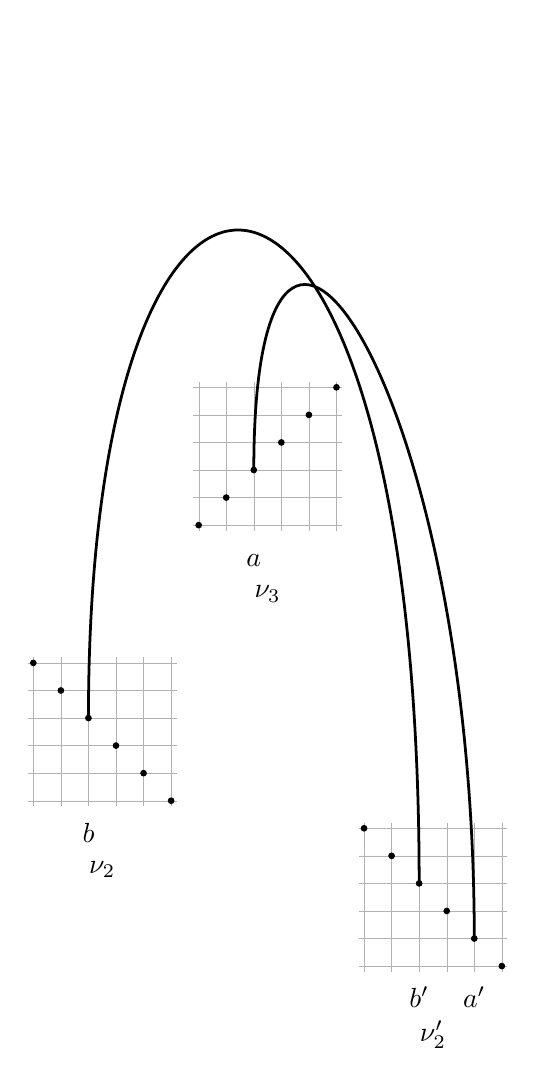
\begin{tikzpicture}
        [
          scale=0.35,
          label/.style={anchor=base}
        ]
        % nu_2
        \draw[step=1cm,black!30,ultra thin,fill=black!10] (-0.2,5.8) grid (5.2,11.2);
        \foreach \x/\y in {0/11,1/10,2/9,3/8,4/7,5/6} {
            \draw [fill=black] (\x,\y) circle (0.1);
        }
        % nu_3
        \draw[step=1cm,black!30,ultra thin,fill=black!10] (5.8,15.8) grid (11.2,21.2);
        \foreach \x/\y in {6/16,7/17,8/18,9/19,10/20,11/21} {
            \draw [fill=black] (\x,\y) circle (0.1);
        }
        % nu'_2
        \draw[step=1cm,black!30,ultra thin,fill=black!10] (11.8,-0.2) grid (17.2,5.2);

        \foreach \x/\y in {12/5,13/4,14/3,15/2,16/1,17/0} {
            \draw [fill=black] (\x,\y) circle (0.1);
        }
        % labels
        \node [label] (x) at (2,4.5) {$b$};
        \node [label] (a) at (8,14.5) {$a$};
        \node [label] (xp) at (14,-1.5) {$b'$};
        \node [label] (ap) at (16,-1.5) {$a'$};
        \node (nu1) at (2.5,3.5) {$\nu_2$};
        \node (nu2) at (8.5,13.5) {$\nu_3$};
        \node (nu1') at (14.5,-2.5) {$\nu'_2$};
        % crossings edges
        \draw [line width=1pt]
        (2,9) .. controls +(0,25) and +(0,30) .. (14,3);
        \draw [line width=1pt]
        (8,18) .. controls +(0,15) and +(0,20) .. (16,1);
      \end{tikzpicture}
    \caption{\label{fig:subfig:no (nu_3, nu'_2)-edge}%
      Claim~\ref{claim:no (nu_3, nu'_2)-edge}:
      Assuming a $(\nu_3, \nu'_2)$-edge $(a, b)$ in $\mathcal{M}$.
    }
  \end{figure}

  \begin{claim}
    \label{claim:no (nu_3, nu'_2)-edge}
    There is no $(\nu_3, \nu'_2)$-edge in $\mathcal{M}$.
  \end{claim}

  \begin{proof}[of Claim~\ref{claim:no (nu_3, nu'_2)-edge}]
    Suppose, aiming at a contradiction, that there exists
    $(\nu_3, \nu'_2)$-edge $(a, a')$ in $\mathcal{M}$.
    According to Claim~\ref{claim:(nu_2, nu'_2)-edge}, there
    exists at least one $(\nu_2, \nu'_2)$-edge $(b, b')$ in $\mathcal{M}$.
    Since $\mathcal{M}$ is containment-free (Lemma~\ref{lemma:matching}),
    we have $b' < a'$.
    Therefore,
    we have $\mu(b) < \mu(a)$ (since $\nu_2$ is below $\nu_3$) and
    $\mu(b') > \mu(a')$ (since $\nu'_2$ is decreasing),
    which contradicts our hypothesis about $\mathcal{M}$.
    See Fig.~\ref{fig:subfig:no (nu_3, nu'_2)-edge}.
    \qed
  \end{proof}

  \begin{claim}
    \label{claim:at most one (nu_2, nu_3)-edge}
    There is at most one $(\nu_2, \nu_3)$-edge
    in $\mathcal{M}$.
  \end{claim}

  \begin{proof}[of Claim~\ref{claim:at most one (nu_2, nu_3)-edge}]
    Apply Lemma~\ref{lemma:at most one edge monotone}.
    \qed
  \end{proof}

    We will see soon (upcoming Claim~\ref{claim:all (nu_2, nu'_2)-edges})
    that there exists actually no $(\nu_2, \nu_3)$-edge
    in $\mathcal{M}$.

  \begin{claim}
    \label{claim:no (nu_1, nu_3)-edge and no (nu'_1, nu_3)-edge}
    There is neither a $(\nu_1, \nu_3)$-edge nor a $(\nu'_1, \nu_3)$-edge
    in $\mathcal{M}$.
  \end{claim}

  \begin{proof}[of Claim~\ref{claim:no (nu_1, nu_3)-edge and no (nu'_1, nu_3)-edge}]
    We first prove that there is no $(\nu_1, \nu_3)$-edge in $\mathcal{M}$.
    Indeed, suppose, aiming at a contradiction, that these exists
    a $(\nu_1, \nu_3)$-edge $(a, a')$ in $\mathcal{M}$.
    According to Claim~\ref{claim:(nu_1, nu'_1)-edge},
    there exists a $(\nu_1, \nu'_1)$-edge $(b, b')$ in $\mathcal{M}$.
    Since $\mathcal{M}$ is containment-free, we must have
    $b < a'$.
    Then it follows that
    $\mu(b) < \mu(a)$ (since $\nu_1$ is incresing) and
    $\mu(b') > \mu(a')$ (since $\nu'_1$ is above $\nu_3$),
    which contradicts our hypothesis about $\mathcal{M}$.

    As for no $(\nu_1, \nu_3)$-edges in $\mathcal{M}$, suppose,
    aiming at a contradiction, that these exists
    a $(\nu'_1, \nu_3)$-edge $(a, a')$ in $\mathcal{M}$.
    According to Claim~\ref{claim:(nu_1, nu'_1)-edge},
    there exists a $(\nu_1, \nu'_1)$-edge $(b, b')$ in $\mathcal{M}$.
    Then it follows that
    $\mu(b) < \mu(a)$ (since $\nu_1$ is below $\nu'_1$) and
    $\mu(b') > \mu(a')$ (since $\nu'_1$ is above $\nu_3$),
    which contradicts our hypothesis about $\mathcal{M}$.
    \qed
  \end{proof}

  \begin{claim}
    \label{claim:(nu_3, nu'_3)-edge}
    There exists a $(\nu_3, \nu'_3)$-edge in $\mathcal{M}$.
  \end{claim}

  \begin{proof}[of Claim~\ref{claim:(nu_3, nu'_3)-edge}]
    Suppose, aiming at a contradiction, that there is no
    $(\nu_3, \nu'_3)$-edge in $\mathcal{M}$.
    Combining
    Claim~\ref{claim:no edge below (nu_2, nu'_2)-edge},
    Claim~\ref{claim:no (nu_3, nu'_2)-edge},
    Claim~\ref{claim:at most one (nu_2, nu_3)-edge}
    and Claim~\ref{claim:no (nu_1, nu_3)-edge and no (nu'_1, nu_3)-edge},
    we conclude that $N_3-1$ positions in $\nu_3$ are involved
    in edges of $\mathcal{M}$ that are
    neither ($\nu_1, \nu_3)$-edges,
    nor $(\nu_2, \nu_3)$-edges
    nor $(\nu'_1, \nu_3)$-edges
    nor $(\nu_3, \nu_3)$-edges.
    But $N_3 - 1 > 2N_4 + 2n + 2k + 4$ (the positions left) and hence
    $\mathcal{M}$ is not a perfect matching,
    which contradicts our hypothesis about $\mathcal{M}$.
    \qed
  \end{proof}

  \begin{claim}
    \label{claim:no edge below one (nu_3, nu'_3)-edge}
    There is
    neither a $(\sigma', \sigma')$-edge,
    nor a $(\sigma', \nu_4)$-edge,
    nor a $(\sigma', \nu'_2)$-edge,
    nor a $(\nu_4, \nu_4)$-edge
    nor a $(\nu_4, \nu'_2)$-edge,
    nor a $(\nu'_2, \nu'_2)$-edge
    in $\mathcal{M}$.
  \end{claim}

  \begin{proof}[of Claim~\ref{claim:no edge below one (nu_3, nu'_3)-edge}]
    Combine Claim~\ref{claim:(nu_3, nu'_3)-edge} with the fact that
    $\mathcal{M}$ is containment-free.
    \qed
  \end{proof}

  The next two claims state that $\mathcal{M}$ actually contains
  all $(\nu_1, \nu'_1)$-edges and all $(\nu_2, \nu'_2)$-edges.

  \begin{claim}
    \label{claim:all (nu_1, nu'_1)-edges}
    $\mathcal{M}$ contains $N_1$ pairwise crossing $(\nu_1, \nu'_1)$-edges.
  \end{claim}

  \begin{proof}[of Claim~\ref{claim:all (nu_1, nu'_1)-edges}]
    Suppose, aiming at a contradiction, that
    $\mathcal{M}$ does not contain $N_1$ $(\nu_1, \nu'_1)$-edge.
    Combing Claim~\ref{claim:no (nu_2, nu'_1)-edge} and
    Claim~\ref{claim:no edge below (nu_2, nu'_2)-edge},
    we conclude that there exists a position $a$ in $\nu'_1$ that is
    involded in an edge $(a, a')$ in $\mathcal{M}$ that is
    neither a $(\nu_1, \nu'_1)$-edge,
    nor a $(\nu_2, \nu'_1)$-edge,
    nor a $(\nu'_1, \nu'_1)$-edge.
    (In other words, $a' > 2N_1 + N_2$.)
    Furthermore, according to Claim~\ref{claim:(nu_1, nu'_1)-edge},
    there exists a $(\nu_1, \nu'_1)$-edge $(x, x')$ in $\mathcal{M}$.
    Then, we have
    $\mu(x) < \mu(a)$ (since $\nu_1$ is below $\nu'_1$) and
    $\mu(x') < \mu(a')$ (since $\nu'_1$ is above any other gadget),
    which contradicts our hypothesis about $\mathcal{M}$.
    \qed
  \end{proof}

  \begin{claim}
    \label{claim:all (nu_2, nu'_2)-edges}
    $\mathcal{M}$ contains $N_2$ pairwise crossing $(\nu_2, \nu'_2)$-edges.
  \end{claim}

  \begin{proof}[of Claim~\ref{claim:all (nu_2, nu'_2)-edges}]
    The key idea is to focus on $\nu'_2$.
    Combining Claim~\ref{claim:no (nu_3, nu'_2)-edge},
    Claim~\ref{claim: no edge right of nu'_2} and
    Claim~\ref{claim:no edge below one (nu_3, nu'_3)-edge},
    we obtain that every position in $\nu'_2$ is involved in
    either a $(\nu_1, \nu'_2$)-edge
    or a $(\nu'_1, \nu'_2$)-edge
    or $(\nu_2, \nu'_2$)-edge.
    But, according to Claim~\ref{claim:all (nu_1, nu'_1)-edges},
    all positions in $\nu_1$ and $\nu'_1$ are involved in
    $(\nu_1, \nu'_1)$-edges.
    Then it follows that
    all positions in $\nu'_2$ are involved in a $(\nu_2, \nu'_2)$,
    and hence
    $\mathcal{M}$ contains $N_2$ pairwise crossing $(\nu_2, \nu'_2)$-edges.
    \qed
  \end{proof}

  \begin{claim}
    \label{claim:no (nu_2, nu_4)-edge}
    There is no $(\nu_2, \nu_4)$-edge in $\mathcal{M}$.
  \end{claim}

  \begin{proof}[of Claim~\ref{claim:no (nu_2, nu_4)-edge}]
    According to Claim~\ref{claim:all (nu_2, nu'_2)-edges},
    all positions in $\nu_2$ and $\nu'_2$ are involved in
    $(\nu_2, \nu'_2)$-edges in $\mathcal{M}$.
    \qed
  \end{proof}

  \begin{claim}
    \label{claim:no (nu_4, nu'_3)-edge}
    There is no $(\nu_4, \nu'_3)$-edge in $\mathcal{M}$.
  \end{claim}

  \begin{proof}[of Claim~\ref{claim:no (nu_4, nu'_3)-edge}]
    Suppose, aiming at a contradiction, that there exists
    a $(\nu_4, \nu'_3)$-edge $(a, a')$ in $\mathcal{M}$.
    According to Claim~\ref{claim:(nu_3, nu'_3)-edge},
    there exists a $(\nu_3, \nu'_3)$-edge $(x, x')$
    in $\mathcal{M}$.
    Since $\mathcal{M}$ is containment-free, we must have
    $x' < a'$.
    Therefore,
    we have $\mu(x) > \mu(a)$ (since $\nu_3$ is above $\nu_4$) and
    $\mu(x') < \nu(a')$ (since $\nu'_3$ is increasing),
    which contradicts our hypothesis about $\mathcal{M}$.
    \qed
  \end{proof}

  \begin{claim}
    \label{claim:(nu_4, nu'_4)-edge}
    There is at least one $(\nu_4, \nu'_4)$-edge in $\mathcal{M}$.
  \end{claim}

  \begin{proof}[of Claim~\ref{claim:(nu_4, nu'_4)-edge}]
    Suppose, aiming at a contradiction, that there is no
    $(\nu_4, \nu'_4)$-edge in $\mathcal{M}$.
    First, according to
    Claim~\ref{claim:all (nu_1, nu'_1)-edges} and
    Claim~\ref{claim:all (nu_2, nu'_2)-edges},
    there is neither a $(\nu_1, \nu_4)$-edge
    nor a $(\nu'_1, \nu_4)$-edge
    nor a $(\nu_2, \nu_4)$-edge
    nor a $(\nu_4, \nu'_2)$-edge in $\mathcal{M}$.
    Furthermore, according to
    Claim~\ref{claim:no edge below (nu_2, nu'_2)-edge} and
    Claim~\ref{claim:no (nu_4, nu'_3)-edge},
    there is neither a $(\nu_3, \nu_4)$-edge
    nor a $(\nu_4, \nu'_3)$-edge in $\mathcal{M}$.
    But $N_4 > 2n + 2k + 2$, and
    hence $\mathcal{M}$ is not perfect,
    which contradicts our hypothesis about $\mathcal{M}$.
    \qed
  \end{proof}

  \begin{claim}
    \label{claim:no edge below (nu_4, nu'_4)-edge}
    There is
    neither a $(\pi', \pi')$-edge
    nor a $(\sigma', \pi'')$-edge
    nor a $(\sigma', \sigma'')$-edge
    in $\mathcal{M}$.
  \end{claim}

  \begin{proof}[of Claim~\ref{claim:no edge below (nu_2, nu'_2)-edge}]
    Combine Claim~\ref{claim:(nu_4, nu'_4)-edge} with the
    fact that $\mathcal{M}$ is containment-free.
    \qed
  \end{proof}

  \begin{claim}
    \label{claim:no (sigma', nu'_3)-edge, no (sigma', nu'_4)-edge}
    There is neither a $(\sigma', \nu'_3)$-edge
    nor a $(\sigma', \nu'_4)$-edge in $\mathcal{M}$.
  \end{claim}

  \begin{proof}[of Claim~\label{claim:no (sigma', nu'_3)-edge}]
    According to
    Claim~\ref{claim: no edge right of nu'_2},
    Claim~\ref{claim:all (nu_1, nu'_1)-edges}
    Claim~\ref{claim:all (nu_2, nu'_2)-edges} and
    Claim~\ref{claim:no (nu_4, nu'_3)-edge}
    every position in $\sigma'$ is involved in
    either a $(\sigma', \nu'_3)$-edge
    or a $(\sigma', \pi')$-edge
    or a $(\sigma', \nu'_4)$-edge
    in $\mathcal{M}$.
    Let $a$ be the first position of $\sigma'$
    (\emph{i.e.}, $a = 2N_1 + N_2 + N_3 + 1$)
    and
    $b$ be the last position of $\sigma'$
    (\emph{i.e.}, $b = 2N_1 + N_2 + N_3 + k + 2$),
    and write $(a, a')$ and $(b, b')$ for the two associated edges of $\mathcal{M}$.
    We consider the presence of a $(\sigma', \nu'_3)$-edge
    or a $(\sigma', \nu'_4)$-edge in $\mathcal{M}$ separately.
    \begin{itemize}
      \item
      Suppose, aiming at a contradiction, that there exists
      a $(\sigma', \nu'_3)$-edge in $\mathcal{M}$.
      Since $\mathcal{M}$ is containment-free, we conclude that
      $(a, a')$ must be a $(\sigma', \nu'_3)$-edge.
      But $\mu(a) = 2N_2 + N_4 + 2n + k + 2 + (k+1) <
      \mu(b) = 2N_2 + N_4 + 2n + k + 2 + (k+2)$, and hence
      $(b, b')$ is also a $(\sigma', \nu'_3)$-edge
      (otherwise we would have $\mu(a') > \mu(b')$ since
      $\nu'_3$ is above $\pi'$ and $\nu'_4$,
      which contradicts our hypothesis).
      Consider any position $c$ but $a$ and $b$ of $\sigma'$
      (\emph{i.e.},
      $a = 2N_1 + N_2 + N_3 + 1 < c < 2N_1 + N_2 + N_3 + k + 2 = b$),
      and let $(c, c')$ be the associate edge in $\mathcal{M}$.
      We first observe that $(c, c')$ is not a $(\sigma', \nu'_3)$-edge,
      since otherwise we would have
      $\mu(a) > \mu(c)$ and $\mu(a') < \mu(c')$
      (since $\mathcal{M}$ is containment-free and $\nu'_3$ is increasing),
      thereby contradicting our hypothesis about $\mathcal{M}$.
      Therefore, $(c, c')$ is either a $(\sigma', \pi)$-edge or a $(\sigma', \nu'_4)$-edge.
      In both cases, $(b, b')$ is contained in $(c, c')$,
      which contradicts our hypothesis about $\mathcal{M}$ being containment-free.
      \item
      Suppose, aiming at a contradiction, that there exists
      a $(\sigma', \nu'_4)$-edge in $\mathcal{M}$.
      Since $\mathcal{M}$ is containment-free, we conclude that
      $(b, b')$ must be a $(\sigma', \nu'_4)$-edge.
      Since there is no $(\sigma', \nu'_3)$-edge in $\mathcal{M}$
      (preceding point),
      $(a, a')$ is either a
      $(\sigma', \pi')$-edge or a $(\sigma', \nu'_4)$-edge.
      In both cases, we have $a' < a$.
      Then it follows that
      $\mu(a) < \mu(b)$
      (since $2N_2 + N_4 + 2n + k + 2 + (k+1) < 2N_2 + N_4 + 2n + k + 2 + (k+2)$)
      and
      $\mu(a') > \mu(b')$ (since $\pi'$ is above $\nu'_4$ if $(a, a')$ is
      a $(\sigma', \pi')$-edge and
      $\nu'_4$ is decreasing if $(a, a')$ is
      a $(\sigma', \nu'_4)$-edge),
      which contradicts our hypothesis about $\mathcal{M}$.
    \end{itemize}
    \qed
  \end{proof}

  Combining the above claims, we conclude that there are
  $k+2$ $(\sigma', \pi')$-edges in $\mathcal{M}$.
  Recall that
  $\sigma' = ((k+1) \; \sigma \; (k+2)) \; [2N_2 + N_4 + 2n + k + 2]$ and that
  $\pi' = ((n+1) \; \pi \; (n+2)) \; [2N_2 + N_4 + n + k + 2]$.
  Then it follows we have
  at least $k$
  %(possibly $k+1$ or $k+2$)
  independent $(\sigma', \pi')$-edges
  $(a, a')$ in $\mathcal{M}$ with
  $2N_1 + N_2 + N_3 + 1 < a < 2N_1 + N_2 + N_3 + k + 2$
  and
  $2N_1 + 2N_2 + 2N_3 + N_4 + (k + 2) + 1 < a' <2N_1 + 2N_2 + 2N_3 + N_4 + (k + 2) + n + 2$.
  Therefore, by our hypothesis about $\mathcal{M}$,
  $\sigma$ occurs as a pattern in $\pi$.
  \qed
\end{proof}

